\chapter{Introduction: Human-Robot interaction and Knowledge}
\label{chapter|introduction}

Robotics is moving from technological demos to real world coworkers/companions.

This shift requires ``awareness'' of humans.

To make informed decision, the robot needs knowledge about the \emph{tasks},
the \emph{environment}, the \emph{situational context}.

\section{The general context of Human-Robot interaction in this work}
\label{sect|general-context}

Interaction for \emph{joint action} in a \emph{situated} environment.

\subsection{A support scenario}
\label{sect|scenario}

\fxnote{Define and describe here from an external point of view a HRI scenario that cover
at minimum all the functions that are covered by the thesis.}

\fxnote{Could be based on/inspired by TUM Kitchen demos}

\subsection{What are the challenges?}
\label{sect|scenario-challenges}

\fxnote{Put focus on knowledge related challenge => focus on questions that need to be
answered}
\fxnote{Show what is difficult in the scenario, and why this requires research.}

\section{Which are the requirements induced by human-robot interaction on knowledge management?}
\label{sect|krs-requirements-hri}

Then, we want to make use of this representation to extend the robot's
\emph{communication function} and \emph{decision function}.

\begin{figure}%[!ht]
\centering
  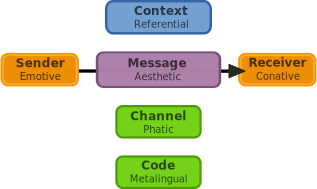
\includegraphics[width=0.6\linewidth]{communication/jakobson_communication_model.pdf}
  \caption{The \emph{Communication Model}, as proposed by Jakobson. In bold
  characters are the \emph{communication dimensions}, in italics, the
  corresponding \emph{communication functions}.}
  \label{fig|jakobson_communication_model}
\end{figure}

\subsection{Main pecularities induced by HRI}
\label{sect|pecularities-krs-for-hri}

Pecularities on knowledge representation required by HRI, in the frame of the
general context defined in section~\ref{sect|general-context}:

\begin{itemize}

	\item Ability to talk about concepts that are not immediately perceived by
	the robot

	\item \fxerror{TBD: absence of knowledge representation} Ability to represent that an agent knows something about
	something else, even if we do not know \emph{what}.

\end{itemize}

\section{Challenges of this thesis}
\label{sect|krs-challenges}

Those two broad targets should lead to two improvements for human-robot
interaction:


\begin{itemize}
	\item to loosen the constraints on symbolic modelling of the robot
	environment by providing more expressive representation system than
	classical databases or fact repositories,

	\item to improve human-robot interaction by explicitely providing to the
	machine an interpretation frame, at least partially shared with the human.

\end{itemize}

The operational targets are two-fold:

\begin{inparaenum}[\itshape a\upshape)]

	\item determine, for a abstract/theoritical/general point of view, how and
	why a cognitive architecture could contribute to these aims; and

	\item implement it.

\end{inparaenum}

\subsection{Targeted applications/experiments}
\label{sect|targeted-applications-experiments}

\begin{itemize}
	\item \textbf{Categorization}: \emph{Odd One Out}-style experiment,
	\item \textbf{Dialogue}: Grounded dialogue,
	\item \textbf{Introspection verbalization}: Integration dialogue/planing, verbalization of plans,
	\fxerror{TDB: integration dialogue/planing + verbalization of plans}
	\item \textbf{Connection to remote knowledge sources}: \emph{DBpedia}, \emph{WordNet}, \emph{KnowRob ontology}...
	\fxerror{TDB: integration remote knowledge sources}
\end{itemize}
